
\begin{frame}
  \frametitle{Computational Methods}
  \begin{figure}[h!]
    \centering
    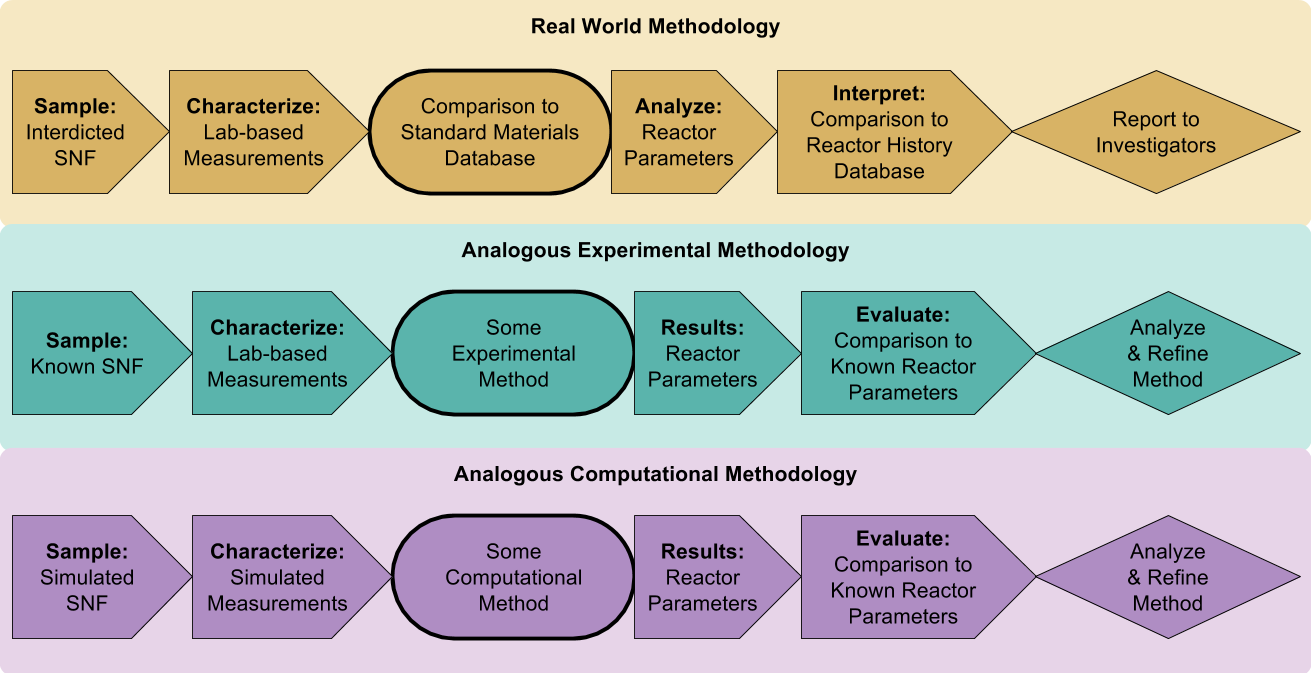
\includegraphics[width=0.9\textwidth]{./figures/ForensicsWorkflows.png}
    \caption{Nuclear forensics research: physical, experimental, and computational}
  \end{figure}
\end{frame}

\begin{frame}
  \frametitle{Computational Methods}
  \begin{figure}[h!]
    \centering
    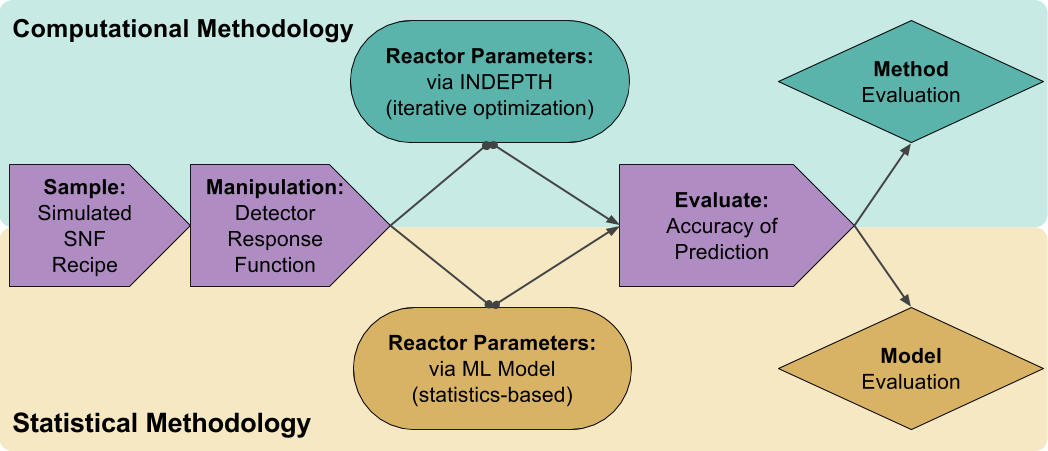
\includegraphics[width=0.9\textwidth]{./figures/CompStatForensicsWorkflow.png}
    \caption{Comparison of two different computational approaches}
  \end{figure}
\end{frame}

\begin{frame}
  \frametitle{Statistical Methods}
  \begin{minipage}{0.5\textwidth}
    \begin{figure}
      \centering
      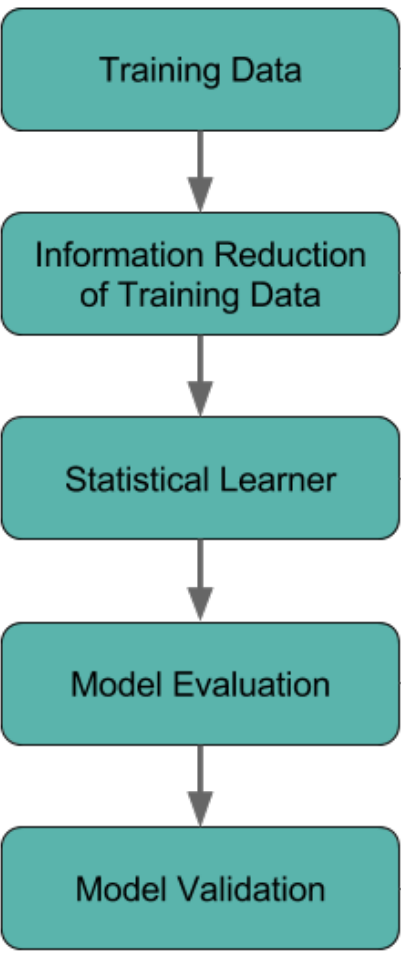
\includegraphics[height=0.6\textheight]{./figures/statmethodology.png}
      \caption{Workflow of a  methodology using statistical models}
    \end{figure}
  \end{minipage}%
  \begin{minipage}{0.5\textwidth}
    \begin{itemize}
      \item Training data: large set of SNF measurements
      \begin{itemize}
        \item Labels (e.g., burnup)
        \item Features (e.g., nuclide concs)
        \item Instances (individual SNF recipe)
      \end{itemize}
      \item Statistical learner
      \begin{itemize}
        \item Machine learning algorithms
        \item Algorithm parameters
        \item Predict label of new instance
      \end{itemize}
      \item Model evaluation
      \begin{itemize}
        \item Diagnostic curves
        \begin{itemize}
          \item Learning curves
          \item Validation curves
        \end{itemize}
        \item Prediction error
        \begin{itemize}
          \item Bias versus variance
          \item Generalizability
        \end{itemize}
      \end{itemize}
    \end{itemize}
  \end{minipage}
\end{frame}

\begin{frame}
  \frametitle{Statistical Methods}
  \begin{figure}[h!]
    \centering
    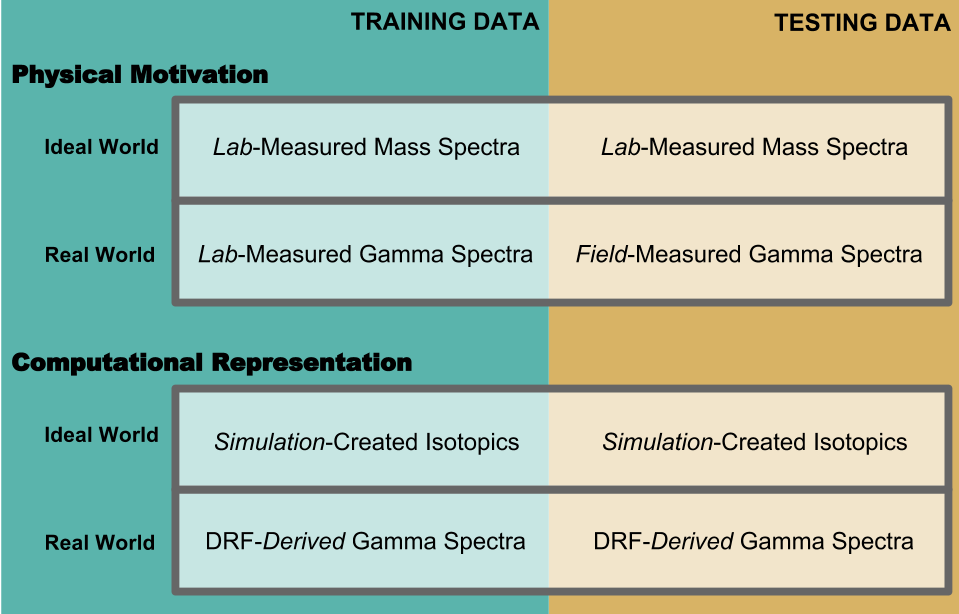
\includegraphics[width=0.75\textwidth]{./figures/proposal.png}
    \caption{Illustration of data set modularity}
  \end{figure}
\end{frame}

